% Useful packages
\documentclass[12pt]{article}
\usepackage[a4paper, left=0.75in, right=0.75in, top=0.75in, bottom=0.75in]{geometry}
\usepackage{amsmath}
\usepackage{amssymb}
\usepackage{float}
\usepackage{tabularx}
\usepackage{array}
\usepackage{multirow}
\usepackage{booktabs}
\usepackage{minted}
\usepackage{xcolor}
\usepackage{enumitem}
\usepackage{hyperref}
\usepackage{graphicx}
\usepackage{longtable}
\usepackage{adjustbox}
\usepackage{textcomp}
\usepackage{subcaption}
\usepackage{mathtools}


% chktex-file 13
% chktex-file 24
% chktex-file 36
% chktex-file 44


% Customizations
\definecolor{inputGray}{HTML}{f8f8f8}
\definecolor{outGray}{HTML}{dfdfdf}


\title{%
    Machine Learning in Computational Biology \\
    \Large Assignment 1 \\
    Bonus Questions
    }
\author{%
    Konstantinos Konstantinidis \\
    Student number: 7115152400017
    }

\begin{document}

\maketitle

\vspace{0.5in}

\textbf{\underline{Repo:}} The repository for this assignment can be found here: \\
\url{https://github.com/KonsKons26/Assignment-1}

\vspace{0.5in}

% \clearpage
% Table of contents
\tableofcontents


\clearpage
%%%%%%%%%%%%%%%%%%%%%%%%%%%%%%%%%%%%%%%%%%%%%%%%%%%%%%%%%%%%%%%%%%%%%%%%%%%%%%%%%%%%
%%%%%%%%%%%%%%%%%%%%%%%%%%%%%%%%%%%%%%%%%%%%%%%%%%%%%%%%%%%%%%%%%%%%%%%%%%%%%%%%%%%%
\section{First bonus task: Using Optuna for hyperparameter tuning}


%%%%%%%%%%%%%%%%%%%%%%%%%%%%%%%%%%%%%%%%%%%%%%%%%%%%%%%%%%%%%%%%%%%%%%%%%%%%%%%%%%%%
\subsection{Migration to Optuna}
Since the \texttt{Regressor} object I had created to perform all regression tasks
was highly modularized, with specific methods for each task, moving from \texttt{%
sklearn}'s \texttt{GridSearchCV} to \texttt{Optuna} was quite simple. I created
a new class named \texttt{RegressorOptuna} which inherited from \texttt{Regressor},
to keep it's basic functionalities the same. Then I modified the private methods
handling each model's hyperparameter optimization to allow me to pass the appropriate
grid spaces --and in the appropriate format-- for \texttt{Optuna} to tune the models.

The objective function \textbf{minimizes} the RMSE of the test set. The sampler
I chose is the \texttt{TPESampler}, a tree-structured Parzen estimator, which fits
one Gaussian Mixture Model (GMM) ($l{x}$) to the set of parameters associated with
the best objective values and another GMM ($g(x)$) to the remaining parameter values.
It chooses the parameter that minimizes the ration $l(x)/g(x)$.

All files are in the appropriate directories, \texttt{src/} and \texttt{notebooks/}
and the models were saved in \texttt{models/bonus1\_optuna/}. Since I used the
features I selected in the previous task, to keep everything organized, the process
includes copying the features files in the \texttt{models/bonus1\_optuna}
directory.

%%%%%%%%%%%%%%%%%%%%%%%%%%%%%%%%%%%%%%%%%%%%%%%%%%%%%%%%%%%%%%%%%%%%%%%%%%%%%%%%%%%%
\subsection{Hyperparameter tuning}
I set the number of trials for each model tuning to $1000$, which seemed appropriate,
as it was not such a demanding number for my machine, and since the hyperparameter
space has so many dimension, I believe that a small number of trials might not be
enough to search the whole space. The complete hyperparameter space, along with the
values chosen by \texttt{Optuna} are shown in Table~\ref{tab:hyperparams}.

\begin{table}[H]
    \centering
    \begin{tabular}{|c|c|c|c|}
        \hline
        \textbf{Model} & \textbf{Parameter} & \textbf{Values} & \textbf{Picked value} \\
        \hline
        \multirow{3}{*}{ElasticNet} 
            & \texttt{$\alpha$} & (0.01, 1.0) & $0.9998$ \\
            & \texttt{l1 ratio} & (0.0, 1.0) & $0.00004$ \\
            & \texttt{tolerance} & [1e-3, 1e-4, 1e-5, 1e-6, 1e-7] & $0.0001$ \\
        \hline
        \multirow{7}{*}{SVR} 
            & \texttt{kernel} & [`rbf', `linear', `poly', `sigmoid'] & `rbf' \\
            & \texttt{degree} & (2, 5) & $2$ \\
            & \texttt{$\gamma$} & [`scale', `auto'] & `auto' \\
            & \texttt{coef\_0} & (0.0, 1) & $0.46631$ \\
            & \texttt{tolerance} & [1e-3, 1e-4, 1e-5, 1e-6, 1e-7] & 1e-6 \\
            & \texttt{C} & (0.1, 10) & $1.49583$ \\
            & \texttt{$\epsilon$} & (0.0, 10.0) & $0.10783$ \\
        \hline
        \multirow{6}{*}{BayesianRidge} 
            & \texttt{tolerance} & [1e-3, 1e-4, 1e-5, 1e-6, 1e-7] & 1e-3 \\
            & \texttt{$\alpha_1$} & (1e-9, 1e-3) & $0.00001$ \\
            & \texttt{$\alpha_2$} & (1e-9, 1e-3) & $0.00001$ \\
            & \texttt{$\lambda_1$} & (1e-3, 1e-9) & $0.00001$ \\
            & \texttt{$\lambda_2$} & (1e-3, 1e-9) & $0.001$ \\
            & \texttt{compute\_score} & [True, False] & True \\
        \hline
    \end{tabular}
    \caption{Hyperparameter spaces for each model.}
    \label{tab:hyperparams}
\end{table}

%%%%%%%%%%%%%%%%%%%%%%%%%%%%%%%%%%%%%%%%%%%%%%%%%%%%%%%%%%%%%%%%%%%%%%%%%%%%%%%%%%%%
\subsection{Results}
After tuning, the best models were saved (along with their scalers, like in the
previous task) and then the validation set was used to measure their performance.
For testing, the same approach with resampling was followed, for $1000$ repeats.
The resulting boxplots are shown in Figure~\ref{fig:optuna}.

\begin{figure}[H]
    \centering
    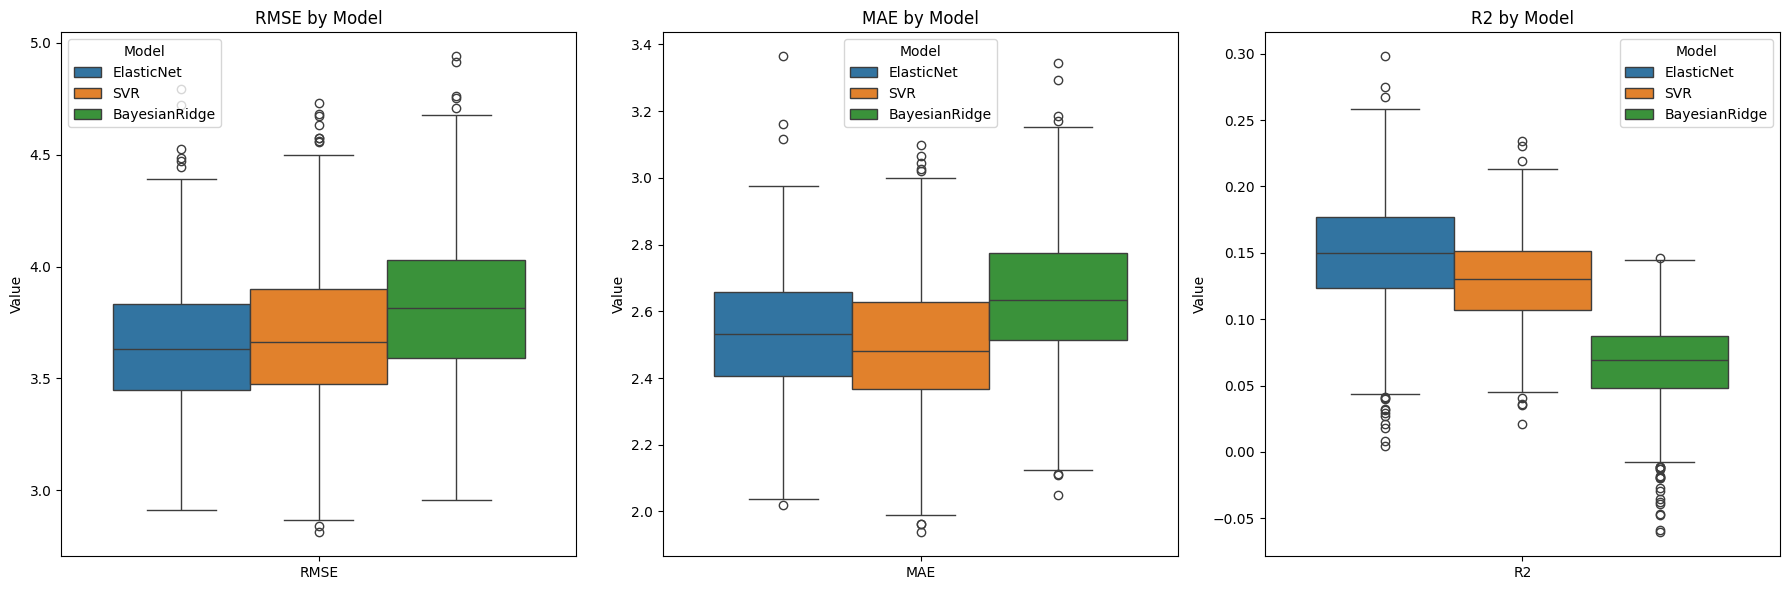
\includegraphics[width=\textwidth]{ims/optuna.png}
    \caption{Test metrics after tuning with \texttt{Optuna}. ElasticNet in blue,
    SVR in orange, and Bayesian Ridge in green.}
    \label{fig:optuna}
\end{figure}

Similar to what was shown in the previous task, Elastic Net is the best performing
model, but its RMSE and MAE still fail to drop below $3$, while $r^2$ fails to
overcome $0.2$. These findings further increase my confidence that this dataset
can not be used for regression tasks, at least no with the models that we analyzed.


\clearpage
%%%%%%%%%%%%%%%%%%%%%%%%%%%%%%%%%%%%%%%%%%%%%%%%%%%%%%%%%%%%%%%%%%%%%%%%%%%%%%%%%%%%
%%%%%%%%%%%%%%%%%%%%%%%%%%%%%%%%%%%%%%%%%%%%%%%%%%%%%%%%%%%%%%%%%%%%%%%%%%%%%%%%%%%%
\section{Second bonus task: Converting the problem to a binary classification task}


%%%%%%%%%%%%%%%%%%%%%%%%%%%%%%%%%%%%%%%%%%%%%%%%%%%%%%%%%%%%%%%%%%%%%%%%%%%%%%%%%%%%
\subsection{Overview}

Converting the target labels (BMI) to binary labels was quite simple. I used the
custom threshold of $25$ to separate the labels into two classes, `overweight'
and `not overweight'. This change happens in-place without the need to store
additional files. The structure of the code base is almost identical to that of the
first task, with the exception of the models (and their corresponding hyperparameter
spaces) used to classify the data. Also, I opted to using \texttt{Optuna} for the
hyperparameter tuning of the models, instead of \texttt{GridSearchCV}.

The way features were selected was the same as in the first task, using the method
that performed the best in classifying the data, based on the following scoring
function (Equation~\ref{eq:score}) which in essence averages out the best accuracy,
precision, recall, and f1 metric.
\begin{equation}    
\text{score} = \frac{
    (\text{mean}(accuracy) + \text{mean}(precision) + \text{mean}(recall) + \text{mean}(f1))
    }{
    4
    }
    \label{eq:score}
\end{equation}

For testing the models, the validation set was used with resampling for $1000$
iterations. Unlike the previous task which involved regression, this task involves
classification, so different metrics must be used. I chose the following metrics
(as provided by \texttt{sklearn}):
\begin{itemize}    
    \item \texttt{accuracy}: The percentage of correct classifications.
    \item \texttt{balanced\_accuracy}: Same as accuracy but takes into account the
    prevalence of each class.
    \item \texttt{precision}: The ratio of true positives over all positives.
    \item \texttt{recall}: The ratio of true positives over true positives and false
    negatives.
    \item \texttt{f1\_score}: The F1 score, can be interpreted as the harmonic
    mean of the precision and recall.
    \item \texttt{roc\_auc}: Compute Area Under the Receiver Operating Characteristic
    Curve (ROC AUC) from prediction scores.
    \item \texttt{average\_precision}: summarizes a precision-recall curve as the
    weighted mean of precisions achieved at each threshold, with the increase in
    recall from the previous threshold used as the weight.
    \item \texttt{confusion\_matrix}: A onfusion matrix.
    \item \texttt{matthews\_corrcoef}: It takes into account true and false positives
    and negatives and is generally regarded as a balanced measure which can be used
    even if the classes are of very different sizes.
\end{itemize}



%%%%%%%%%%%%%%%%%%%%%%%%%%%%%%%%%%%%%%%%%%%%%%%%%%%%%%%%%%%%%%%%%%%%%%%%%%%%%%%%%%%%
\subsection{Feature Selection}

Figure~\ref{fig:classif_features} shows the features selected for each model.
The \texttt{VarianceThreshold} method was used for both of them, with a threshold of
$0.5$. We can see that both models were optimized for exactly the same features.

\begin{figure}[H]
    \centering
    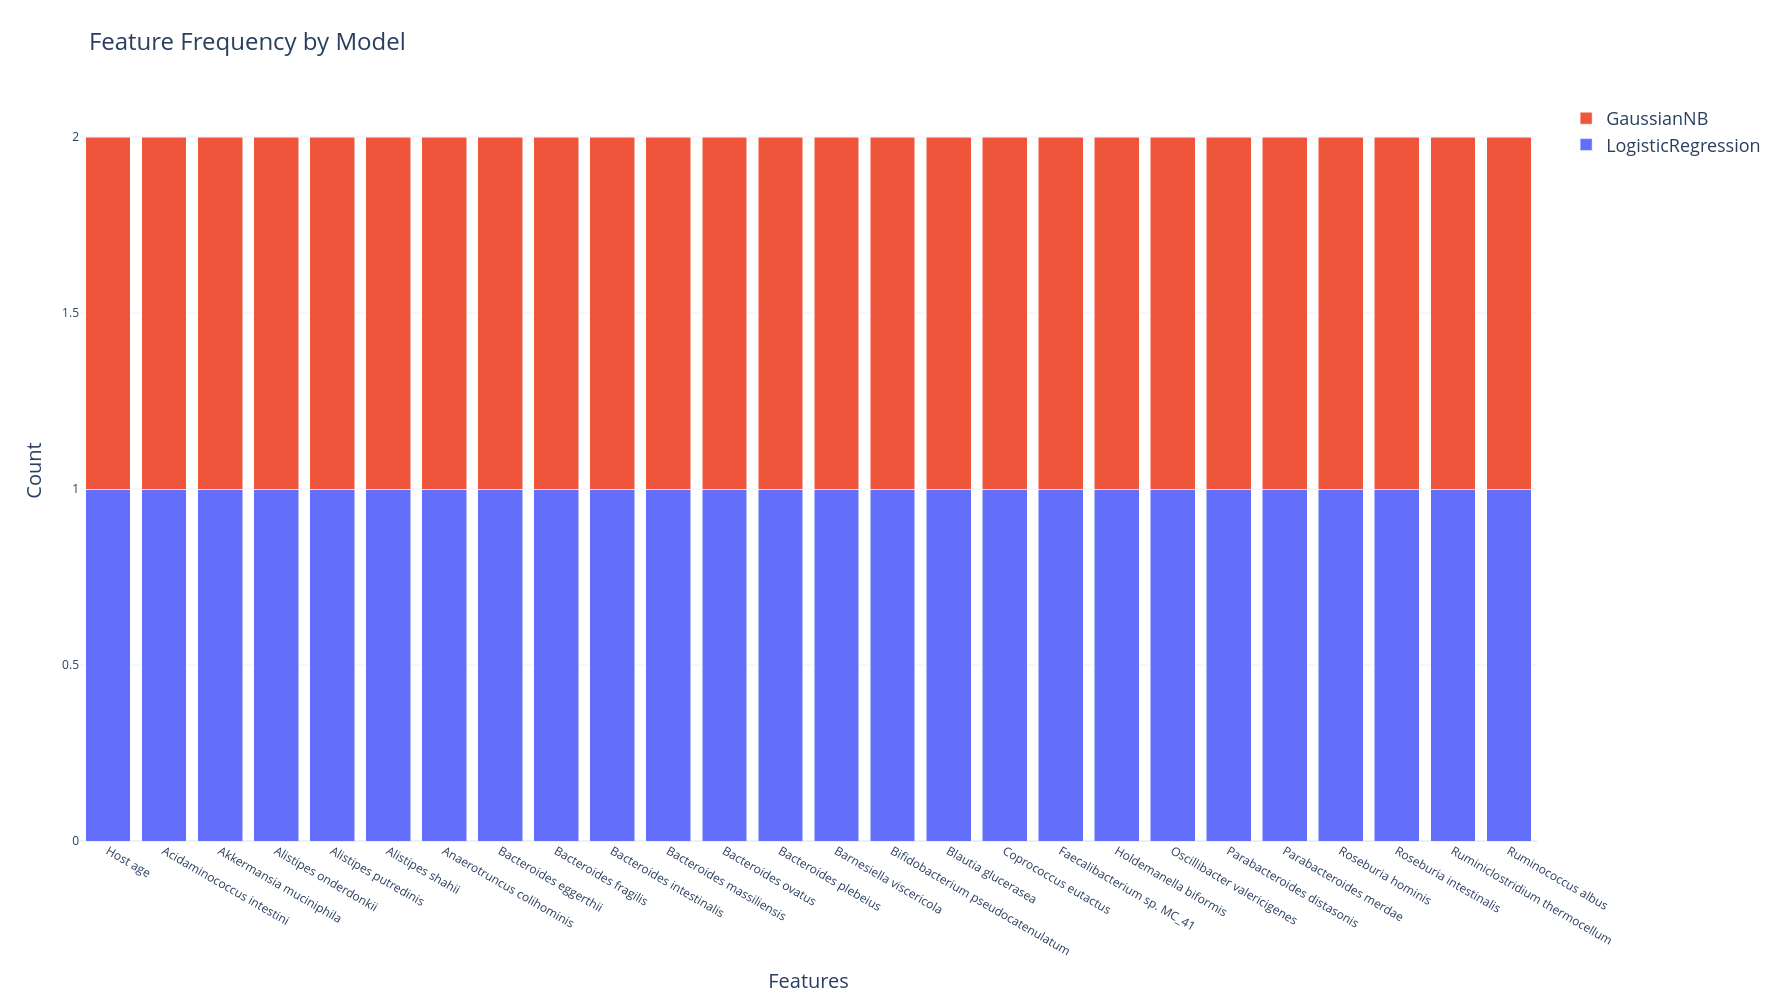
\includegraphics[width=\textwidth]{ims/selected_features_classif.png}
    \caption{Selected features.}
    \label{fig:classif_features}
\end{figure}


%%%%%%%%%%%%%%%%%%%%%%%%%%%%%%%%%%%%%%%%%%%%%%%%%%%%%%%%%%%%%%%%%%%%%%%%%%%%%%%%%%%%
\subsection{Tuning}

Hyperparameter tuning was done using \texttt{Optuna} with cross validation and at
$100$ trials. Table~\ref{tab:hyperparams_classif} summarizes the hyperparameter
grids passed in and the seelcted values by the model. We can see that for the 
Logistic Regression model, the penalty is almost exclusievly L2, the tolerance is
small, and the intercept is fitted. The variance smoothing for the GNB stays at
1e-6 which is the default of the model.

\begin{table}[H]
    \centering
    \begin{tabular}{|c|c|c|c|}
        \hline
        \textbf{Model} & \textbf{Parameter} & \textbf{Values} & \textbf{Picked value} \\
        \hline
        \multirow{7}{*}{Logistic Regression}
            & \texttt{penalty} & ``elasticnet'' & ``elasticnet'' \\
            & \texttt{l1\_ratio} & (0.0, 1.0) & $0.0104$ \\
            & \texttt{tolerance} & (1e-7, 1e-1) & $0.02814$ \\
            & \texttt{C} & (0.001, 1000) & $0.02330$ \\
            & \texttt{fit\_intercept} & [True, False] & True \\
            & \texttt{solver} & ``saga'' & ``saga'' \\
            & \texttt{max\_iter} & ($1000000$, $10000000$) & $5313982$ \\
        \hline
        \multirow{1}{*}{Gaussian Naive Bayes}
            & \texttt{var\_smoothing} & (1e-9, 1e-1) & 1e-6 \\
        \hline
    \end{tabular}
    \caption{Hyperparameter spaces for each model.}
    \label{tab:hyperparams_classif}
\end{table}

%%%%%%%%%%%%%%%%%%%%%%%%%%%%%%%%%%%%%%%%%%%%%%%%%%%%%%%%%%%%%%%%%%%%%%%%%%%%%%%%%%%%
\subsection{Results}

All models (baseline, feature selection, and tuned) are tested using the validation
set. Some of their metrics are presented here (\textit{all plots are presented in
the notebooks}).

The fact that the baseline models are performing better is a strong indication that
something is not working as expected. One issue might be with how I performed
hyperparameter tuning. For each trial I let the objective function internally
perform cross validation and return the mean of the scores, which might be
counterproductive for the \texttt{Optuna} optimizer, a possible solution could be
to perform corss validation outside the hyperparameter optimization loop; a possible
improvement would be to implement that and check if the scores improved.

\begin{figure}[H]
    \centering
    \begin{subfigure}{0.31\textwidth}
        \centering
        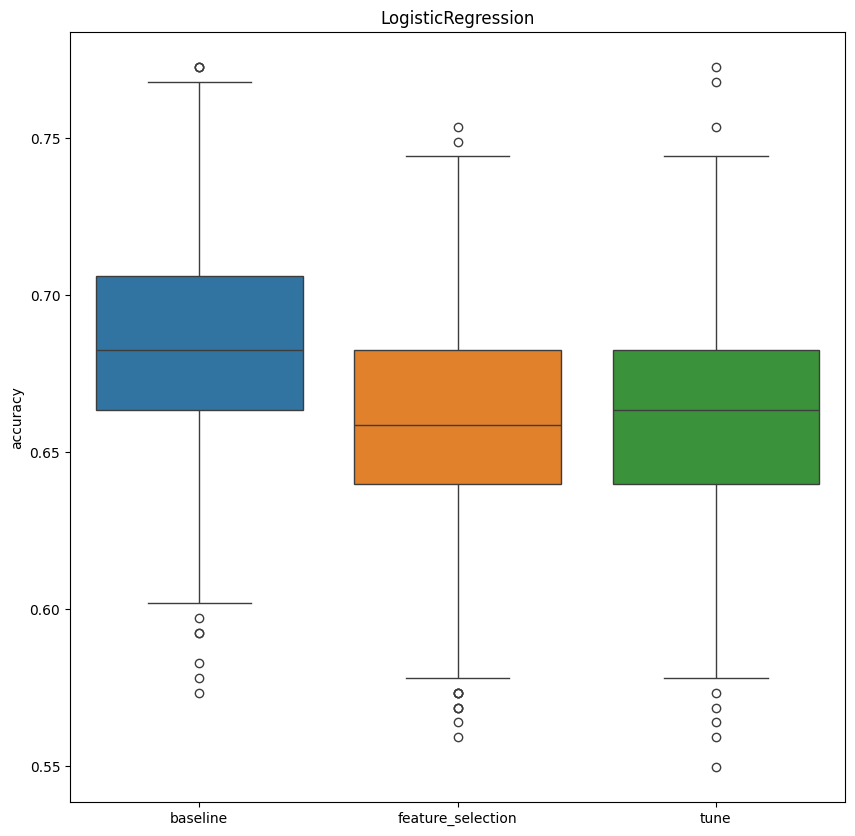
\includegraphics[width=\linewidth]{ims/logreg_accuracy.png}
        \caption{Accuracy}
        \label{fig:logreg_acc}
    \end{subfigure}
    \begin{subfigure}{0.31\textwidth}
        \centering
        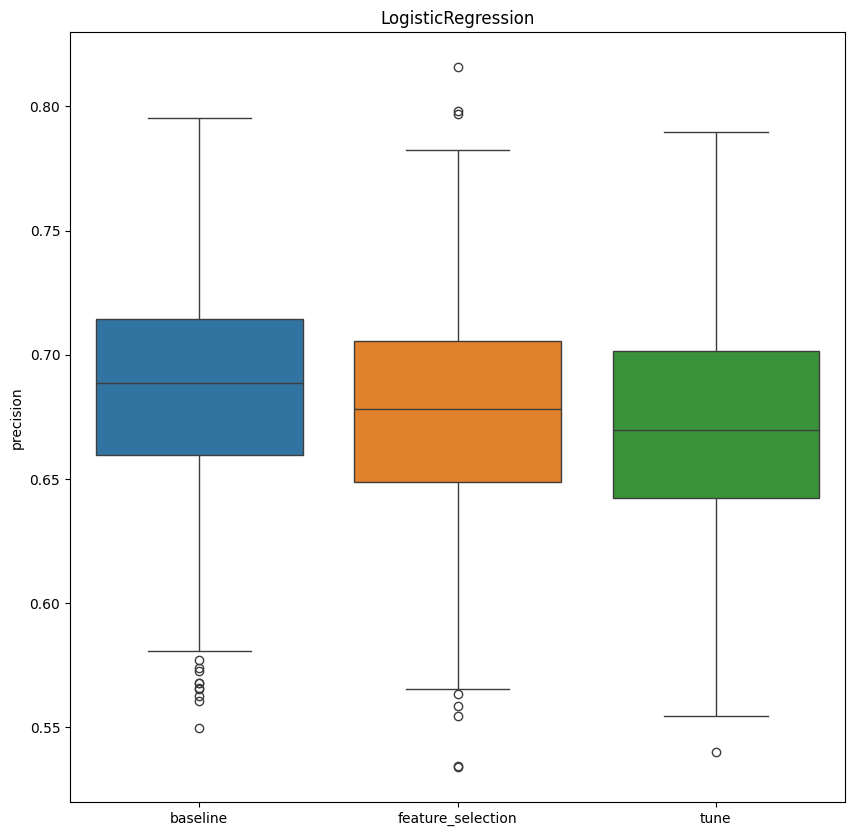
\includegraphics[width=\linewidth]{ims/logreg_precision.png}
        \caption{Precision}
        \label{fig:logreg_prec}
    \end{subfigure}
    \begin{subfigure}{0.31\textwidth}
        \centering
        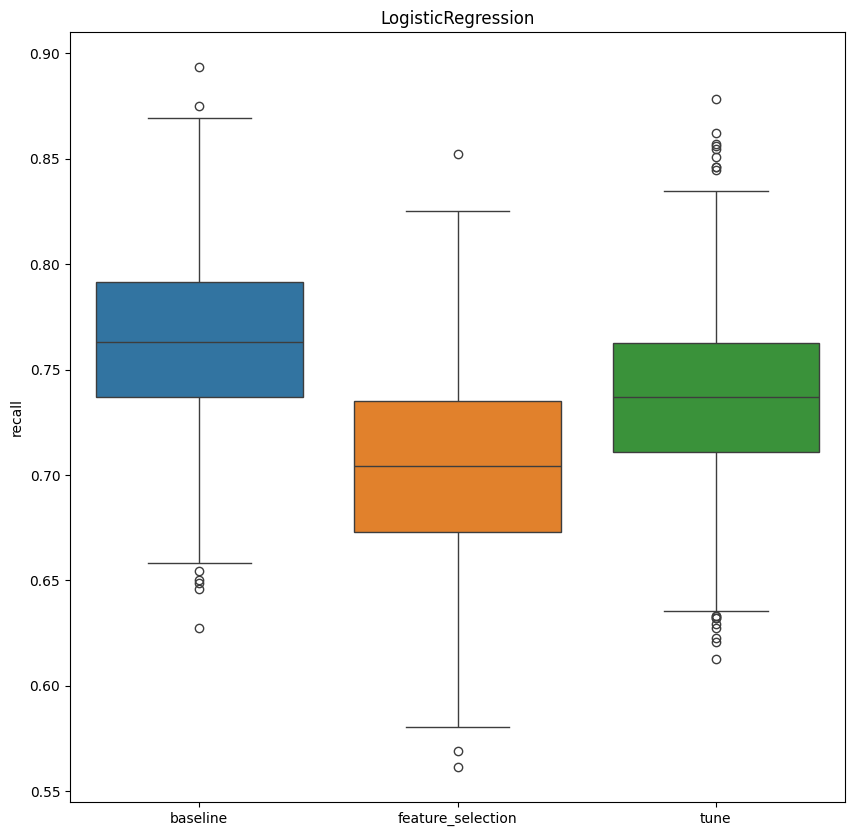
\includegraphics[width=\linewidth]{ims/logreg_recall.png}
        \caption{Recall}
        \label{fig:logreg_rec}
    \end{subfigure}
    \caption{Logistic Regression: Results based on the validation set. Accuracy,
    precision, and recall for the baseline, feature selection, and tuned models
    (baseline in blue, feature selection in orange, and tuned in green).}
    \label{fig:logreg}
\end{figure}

\begin{figure}[H]
    \centering
    \begin{subfigure}{0.31\textwidth}
        \centering
        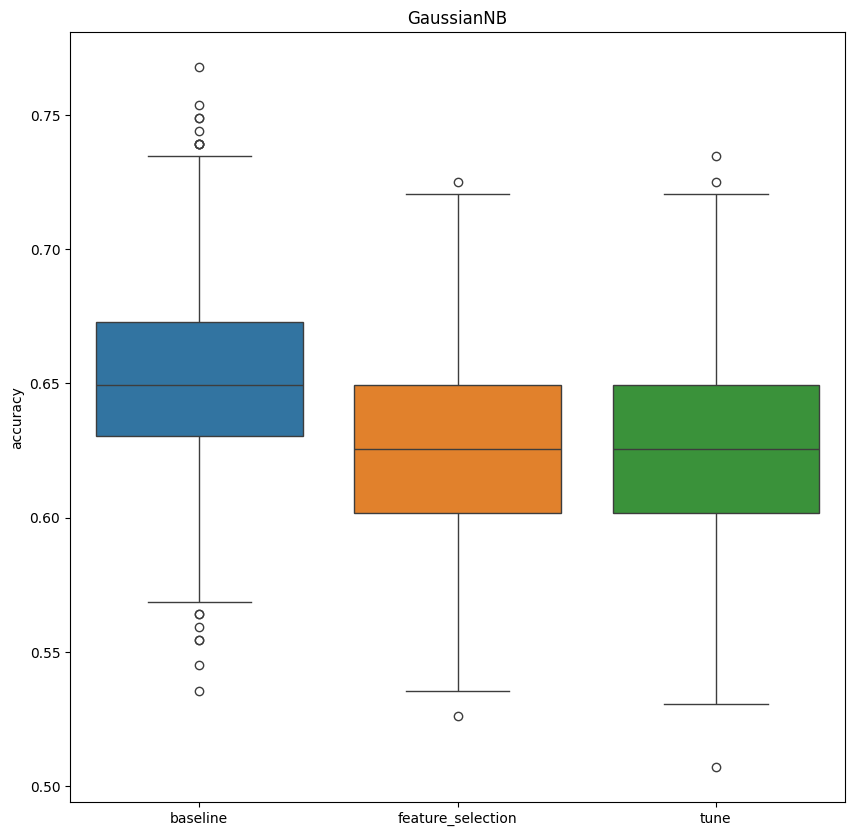
\includegraphics[width=\linewidth]{ims/gnb_accuracy.png}
        \caption{Accuracy}
        \label{fig:gnb_acc}
    \end{subfigure}
    \begin{subfigure}{0.31\textwidth}
        \centering
        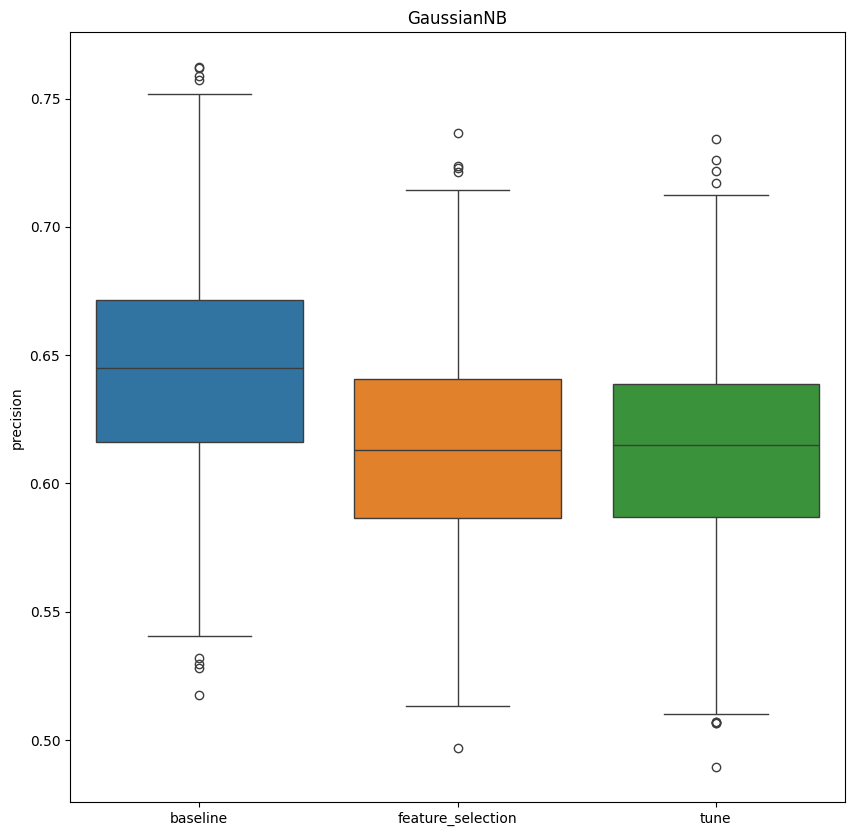
\includegraphics[width=\linewidth]{ims/gnb_precision.png}
        \caption{Precision}
        \label{fig:gnb_prec}
    \end{subfigure}
    \begin{subfigure}{0.31\textwidth}
        \centering
        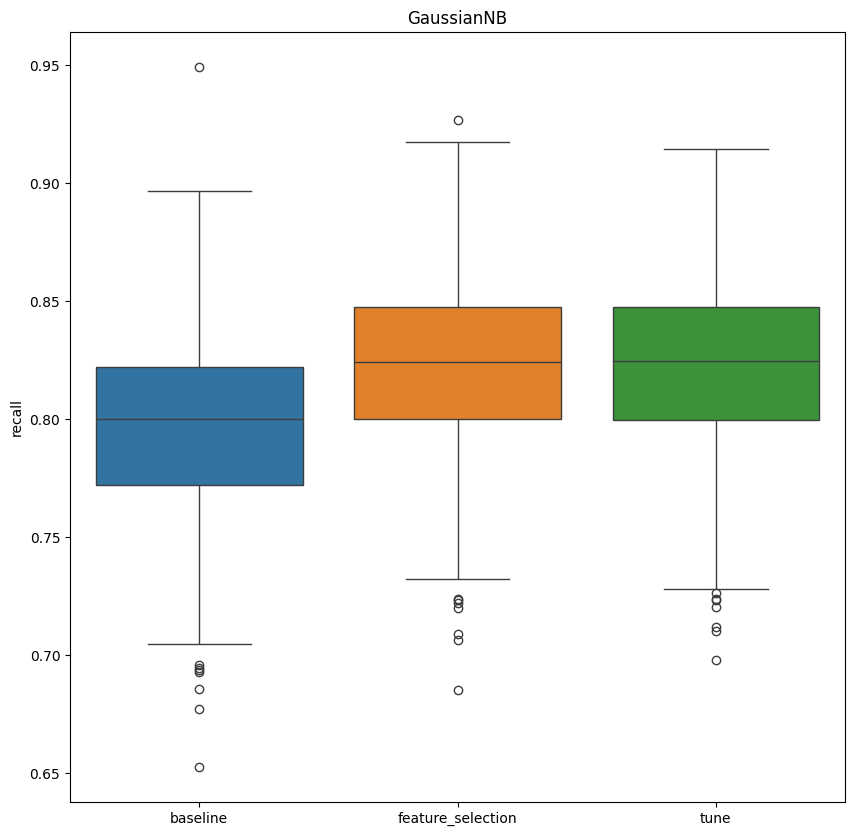
\includegraphics[width=\linewidth]{ims/gnb_recall.png}
        \caption{Recall}
        \label{fig:gnb_rec}
    \end{subfigure}
    \caption{Gaussian Naive Bayes: Results based on the validation set. Accuracy,
    precision, and recall for the baseline, feature selection, and tuned models
    (baseline in blue, feature selection in orange, and tuned in green).}
    \label{fig:gnb}
\end{figure}


\end{document}